\documentclass[]{article}
\usepackage{lmodern}
\usepackage{amssymb,amsmath}
\usepackage{ifxetex,ifluatex}
\usepackage{fixltx2e} % provides \textsubscript
\ifnum 0\ifxetex 1\fi\ifluatex 1\fi=0 % if pdftex
  \usepackage[T1]{fontenc}
  \usepackage[utf8]{inputenc}
\else % if luatex or xelatex
  \ifxetex
    \usepackage{mathspec}
  \else
    \usepackage{fontspec}
  \fi
  \defaultfontfeatures{Ligatures=TeX,Scale=MatchLowercase}
\fi
% use upquote if available, for straight quotes in verbatim environments
\IfFileExists{upquote.sty}{\usepackage{upquote}}{}
% use microtype if available
\IfFileExists{microtype.sty}{%
\usepackage{microtype}
\UseMicrotypeSet[protrusion]{basicmath} % disable protrusion for tt fonts
}{}
\usepackage[margin=1in]{geometry}
\usepackage{hyperref}
\hypersetup{unicode=true,
            pdftitle={561\_notes},
            pdfauthor={Shivam Verma},
            pdfborder={0 0 0},
            breaklinks=true}
\urlstyle{same}  % don't use monospace font for urls
\usepackage{color}
\usepackage{fancyvrb}
\newcommand{\VerbBar}{|}
\newcommand{\VERB}{\Verb[commandchars=\\\{\}]}
\DefineVerbatimEnvironment{Highlighting}{Verbatim}{commandchars=\\\{\}}
% Add ',fontsize=\small' for more characters per line
\usepackage{framed}
\definecolor{shadecolor}{RGB}{248,248,248}
\newenvironment{Shaded}{\begin{snugshade}}{\end{snugshade}}
\newcommand{\AlertTok}[1]{\textcolor[rgb]{0.94,0.16,0.16}{#1}}
\newcommand{\AnnotationTok}[1]{\textcolor[rgb]{0.56,0.35,0.01}{\textbf{\textit{#1}}}}
\newcommand{\AttributeTok}[1]{\textcolor[rgb]{0.77,0.63,0.00}{#1}}
\newcommand{\BaseNTok}[1]{\textcolor[rgb]{0.00,0.00,0.81}{#1}}
\newcommand{\BuiltInTok}[1]{#1}
\newcommand{\CharTok}[1]{\textcolor[rgb]{0.31,0.60,0.02}{#1}}
\newcommand{\CommentTok}[1]{\textcolor[rgb]{0.56,0.35,0.01}{\textit{#1}}}
\newcommand{\CommentVarTok}[1]{\textcolor[rgb]{0.56,0.35,0.01}{\textbf{\textit{#1}}}}
\newcommand{\ConstantTok}[1]{\textcolor[rgb]{0.00,0.00,0.00}{#1}}
\newcommand{\ControlFlowTok}[1]{\textcolor[rgb]{0.13,0.29,0.53}{\textbf{#1}}}
\newcommand{\DataTypeTok}[1]{\textcolor[rgb]{0.13,0.29,0.53}{#1}}
\newcommand{\DecValTok}[1]{\textcolor[rgb]{0.00,0.00,0.81}{#1}}
\newcommand{\DocumentationTok}[1]{\textcolor[rgb]{0.56,0.35,0.01}{\textbf{\textit{#1}}}}
\newcommand{\ErrorTok}[1]{\textcolor[rgb]{0.64,0.00,0.00}{\textbf{#1}}}
\newcommand{\ExtensionTok}[1]{#1}
\newcommand{\FloatTok}[1]{\textcolor[rgb]{0.00,0.00,0.81}{#1}}
\newcommand{\FunctionTok}[1]{\textcolor[rgb]{0.00,0.00,0.00}{#1}}
\newcommand{\ImportTok}[1]{#1}
\newcommand{\InformationTok}[1]{\textcolor[rgb]{0.56,0.35,0.01}{\textbf{\textit{#1}}}}
\newcommand{\KeywordTok}[1]{\textcolor[rgb]{0.13,0.29,0.53}{\textbf{#1}}}
\newcommand{\NormalTok}[1]{#1}
\newcommand{\OperatorTok}[1]{\textcolor[rgb]{0.81,0.36,0.00}{\textbf{#1}}}
\newcommand{\OtherTok}[1]{\textcolor[rgb]{0.56,0.35,0.01}{#1}}
\newcommand{\PreprocessorTok}[1]{\textcolor[rgb]{0.56,0.35,0.01}{\textit{#1}}}
\newcommand{\RegionMarkerTok}[1]{#1}
\newcommand{\SpecialCharTok}[1]{\textcolor[rgb]{0.00,0.00,0.00}{#1}}
\newcommand{\SpecialStringTok}[1]{\textcolor[rgb]{0.31,0.60,0.02}{#1}}
\newcommand{\StringTok}[1]{\textcolor[rgb]{0.31,0.60,0.02}{#1}}
\newcommand{\VariableTok}[1]{\textcolor[rgb]{0.00,0.00,0.00}{#1}}
\newcommand{\VerbatimStringTok}[1]{\textcolor[rgb]{0.31,0.60,0.02}{#1}}
\newcommand{\WarningTok}[1]{\textcolor[rgb]{0.56,0.35,0.01}{\textbf{\textit{#1}}}}
\usepackage{graphicx,grffile}
\makeatletter
\def\maxwidth{\ifdim\Gin@nat@width>\linewidth\linewidth\else\Gin@nat@width\fi}
\def\maxheight{\ifdim\Gin@nat@height>\textheight\textheight\else\Gin@nat@height\fi}
\makeatother
% Scale images if necessary, so that they will not overflow the page
% margins by default, and it is still possible to overwrite the defaults
% using explicit options in \includegraphics[width, height, ...]{}
\setkeys{Gin}{width=\maxwidth,height=\maxheight,keepaspectratio}
\IfFileExists{parskip.sty}{%
\usepackage{parskip}
}{% else
\setlength{\parindent}{0pt}
\setlength{\parskip}{6pt plus 2pt minus 1pt}
}
\setlength{\emergencystretch}{3em}  % prevent overfull lines
\providecommand{\tightlist}{%
  \setlength{\itemsep}{0pt}\setlength{\parskip}{0pt}}
\setcounter{secnumdepth}{0}
% Redefines (sub)paragraphs to behave more like sections
\ifx\paragraph\undefined\else
\let\oldparagraph\paragraph
\renewcommand{\paragraph}[1]{\oldparagraph{#1}\mbox{}}
\fi
\ifx\subparagraph\undefined\else
\let\oldsubparagraph\subparagraph
\renewcommand{\subparagraph}[1]{\oldsubparagraph{#1}\mbox{}}
\fi

%%% Use protect on footnotes to avoid problems with footnotes in titles
\let\rmarkdownfootnote\footnote%
\def\footnote{\protect\rmarkdownfootnote}

%%% Change title format to be more compact
\usepackage{titling}

% Create subtitle command for use in maketitle
\providecommand{\subtitle}[1]{
  \posttitle{
    \begin{center}\large#1\end{center}
    }
}

\setlength{\droptitle}{-2em}

  \title{561\_notes}
    \pretitle{\vspace{\droptitle}\centering\huge}
  \posttitle{\par}
    \author{Shivam Verma}
    \preauthor{\centering\large\emph}
  \postauthor{\par}
      \predate{\centering\large\emph}
  \postdate{\par}
    \date{15/12/2019}


\begin{document}
\maketitle

\begin{center}\rule{0.5\linewidth}{\linethickness}\end{center}

F statistic is also called (Coefficient of partial determination)\\
-
\href{https://en.wikipedia.org/wiki/Coefficient_of_determination}{see:}\\
-
\href{http://facweb.cs.depaul.edu/sjost/csc423/documents/f-test-reg.htm}{See
also}\\
- The formula:
\texttt{((SS\_res\_reduced-SS\_res\_full)/k)/(SS\_res\_full/(n-p-1))}.\\
* \texttt{k} is number of parameters which is different\\
* \texttt{p} is number of parameters in the full model\\
* \texttt{n} is number of rows in the dataset

\begin{Shaded}
\begin{Highlighting}[]
\NormalTok{gpa_data <-}\StringTok{ }\KeywordTok{read_csv}\NormalTok{(}\StringTok{"C:/MyDisk/MDS/DSCI_561/DSCI_561_lab3_sverma92/gpa_data.csv"}\NormalTok{)}
\end{Highlighting}
\end{Shaded}

\begin{verbatim}
## Parsed with column specification:
## cols(
##   high_gpa = col_double(),
##   math_sat = col_double(),
##   verb_sat = col_double(),
##   univ_gpa = col_double()
## )
\end{verbatim}

\begin{Shaded}
\begin{Highlighting}[]
\NormalTok{model_}\DecValTok{1}\NormalTok{ <-}\StringTok{ }\KeywordTok{lm}\NormalTok{(univ_gpa}\OperatorTok{~}\NormalTok{high_gpa, gpa_data)}
\NormalTok{model_}\DecValTok{2}\NormalTok{ <-}\StringTok{ }\KeywordTok{lm}\NormalTok{(univ_gpa}\OperatorTok{~}\NormalTok{high_gpa}\OperatorTok{+}\NormalTok{math_sat, gpa_data)}

\CommentTok{####}
\CommentTok{# Comparing model1 with null intercept only model}
\NormalTok{SS_res_reduced <-}\StringTok{ }\KeywordTok{sum}\NormalTok{((gpa_data}\OperatorTok{$}\NormalTok{univ_gpa }\OperatorTok{-}\StringTok{ }\KeywordTok{mean}\NormalTok{(gpa_data}\OperatorTok{$}\NormalTok{univ_gpa))}\OperatorTok{^}\DecValTok{2}\NormalTok{)}
\NormalTok{SS_res_full <-}\StringTok{ }\KeywordTok{sum}\NormalTok{((broom}\OperatorTok{::}\KeywordTok{augment}\NormalTok{(model_}\DecValTok{1}\NormalTok{)}\OperatorTok{$}\NormalTok{.resid)}\OperatorTok{^}\DecValTok{2}\NormalTok{)}
\NormalTok{k <-}\StringTok{ }\DecValTok{1}
\NormalTok{n <-}\StringTok{ }\KeywordTok{nrow}\NormalTok{(gpa_data)}
\NormalTok{p <-}\StringTok{ }\DecValTok{1}

\NormalTok{F_stas <-}\StringTok{ }\NormalTok{((SS_res_reduced }\OperatorTok{-}\StringTok{ }\NormalTok{SS_res_full)}\OperatorTok{/}\NormalTok{k)}\OperatorTok{/}\NormalTok{(SS_res_full}\OperatorTok{/}\NormalTok{(n}\OperatorTok{-}\NormalTok{p}\DecValTok{-1}\NormalTok{))}
\KeywordTok{anova}\NormalTok{(}\KeywordTok{lm}\NormalTok{(univ_gpa}\OperatorTok{~}\DecValTok{1}\NormalTok{, gpa_data), model_}\DecValTok{1}\NormalTok{)}
\end{Highlighting}
\end{Shaded}

\begin{verbatim}
## Analysis of Variance Table
## 
## Model 1: univ_gpa ~ 1
## Model 2: univ_gpa ~ high_gpa
##   Res.Df     RSS Df Sum of Sq      F    Pr(>F)    
## 1    104 20.7981                                  
## 2    103  8.1587  1    12.639 159.57 < 2.2e-16 ***
## ---
## Signif. codes:  0 '***' 0.001 '**' 0.01 '*' 0.05 '.' 0.1 ' ' 1
\end{verbatim}

\begin{Shaded}
\begin{Highlighting}[]
\CommentTok{# Comparing model2 with null intercept only model}
\NormalTok{SS_res_full <-}\StringTok{ }\KeywordTok{sum}\NormalTok{((broom}\OperatorTok{::}\KeywordTok{augment}\NormalTok{(model_}\DecValTok{2}\NormalTok{)}\OperatorTok{$}\NormalTok{.resid)}\OperatorTok{^}\DecValTok{2}\NormalTok{)}
\NormalTok{k <-}\StringTok{ }\DecValTok{2}
\NormalTok{n <-}\StringTok{ }\KeywordTok{nrow}\NormalTok{(gpa_data)}
\NormalTok{p <-}\StringTok{ }\DecValTok{2}

\NormalTok{F_stas <-}\StringTok{ }\NormalTok{((SS_res_reduced }\OperatorTok{-}\StringTok{ }\NormalTok{SS_res_full)}\OperatorTok{/}\NormalTok{k)}\OperatorTok{/}\NormalTok{(SS_res_full}\OperatorTok{/}\NormalTok{(n}\OperatorTok{-}\NormalTok{p}\DecValTok{-1}\NormalTok{))}
\KeywordTok{anova}\NormalTok{(}\KeywordTok{lm}\NormalTok{(univ_gpa}\OperatorTok{~}\DecValTok{1}\NormalTok{, gpa_data), model_}\DecValTok{2}\NormalTok{)}
\end{Highlighting}
\end{Shaded}

\begin{verbatim}
## Analysis of Variance Table
## 
## Model 1: univ_gpa ~ 1
## Model 2: univ_gpa ~ high_gpa + math_sat
##   Res.Df     RSS Df Sum of Sq      F    Pr(>F)    
## 1    104 20.7981                                  
## 2    102  7.9511  2    12.847 82.403 < 2.2e-16 ***
## ---
## Signif. codes:  0 '***' 0.001 '**' 0.01 '*' 0.05 '.' 0.1 ' ' 1
\end{verbatim}

\begin{Shaded}
\begin{Highlighting}[]
\CommentTok{# Comparing model2 with model1}
\NormalTok{SS_res_reduced <-}\StringTok{ }\KeywordTok{sum}\NormalTok{((broom}\OperatorTok{::}\KeywordTok{augment}\NormalTok{(model_}\DecValTok{1}\NormalTok{)}\OperatorTok{$}\NormalTok{.resid)}\OperatorTok{^}\DecValTok{2}\NormalTok{)}
\NormalTok{k <-}\StringTok{ }\DecValTok{1}
\NormalTok{n <-}\StringTok{ }\KeywordTok{nrow}\NormalTok{(gpa_data)}
\NormalTok{p <-}\StringTok{ }\DecValTok{2}

\NormalTok{F_stas <-}\StringTok{ }\NormalTok{((SS_res_reduced }\OperatorTok{-}\StringTok{ }\NormalTok{SS_res_full)}\OperatorTok{/}\NormalTok{k)}\OperatorTok{/}\NormalTok{(SS_res_full}\OperatorTok{/}\NormalTok{(n}\OperatorTok{-}\NormalTok{p}\DecValTok{-1}\NormalTok{))}
\KeywordTok{anova}\NormalTok{(model_}\DecValTok{1}\NormalTok{, model_}\DecValTok{2}\NormalTok{)}
\end{Highlighting}
\end{Shaded}

\begin{verbatim}
## Analysis of Variance Table
## 
## Model 1: univ_gpa ~ high_gpa
## Model 2: univ_gpa ~ high_gpa + math_sat
##   Res.Df    RSS Df Sum of Sq      F Pr(>F)
## 1    103 8.1587                           
## 2    102 7.9511  1   0.20759 2.6631 0.1058
\end{verbatim}

\begin{Shaded}
\begin{Highlighting}[]
\CommentTok{####}

\KeywordTok{print}\NormalTok{(}\KeywordTok{paste}\NormalTok{(}\StringTok{"The t-statistic from tidy is:"}\NormalTok{, }\KeywordTok{round}\NormalTok{(}\KeywordTok{tidy}\NormalTok{(model_}\DecValTok{2}\NormalTok{)}\OperatorTok{$}\NormalTok{statistic[}\DecValTok{3}\NormalTok{], }\DataTypeTok{digits=}\DecValTok{3}\NormalTok{), }\StringTok{"square of which is:"}\NormalTok{, }\KeywordTok{round}\NormalTok{(}\KeywordTok{tidy}\NormalTok{(model_}\DecValTok{2}\NormalTok{)}\OperatorTok{$}\NormalTok{statistic[}\DecValTok{3}\NormalTok{]}\OperatorTok{^}\DecValTok{2}\NormalTok{, }\DataTypeTok{digits=}\DecValTok{3}\NormalTok{)))}
\end{Highlighting}
\end{Shaded}

\begin{verbatim}
## [1] "The t-statistic from tidy is: 1.632 square of which is: 2.663"
\end{verbatim}

\begin{Shaded}
\begin{Highlighting}[]
\KeywordTok{print}\NormalTok{(}\KeywordTok{paste}\NormalTok{(}\StringTok{"The F-statistic from anova is:"}\NormalTok{, }\KeywordTok{round}\NormalTok{(}\KeywordTok{tidy}\NormalTok{(}\KeywordTok{anova}\NormalTok{(model_}\DecValTok{1}\NormalTok{, model_}\DecValTok{2}\NormalTok{))}\OperatorTok{$}\NormalTok{statistic[}\DecValTok{2}\NormalTok{], }\DataTypeTok{digits=}\DecValTok{3}\NormalTok{)))}
\end{Highlighting}
\end{Shaded}

\begin{verbatim}
## Warning: Unknown or uninitialised column: 'term'.
\end{verbatim}

\begin{verbatim}
## [1] "The F-statistic from anova is: 2.663"
\end{verbatim}

\begin{quote}
In the special case of comparing the two exact same hypotheses in a
least squares linear model, it can be shown that the F-statistic is
equal to the T-statistic squared, and that the p-value of the F-test and
T-test are equal (see
\href{https://canovasjm.netlify.com/2018/10/29/when-does-the-f-test-reduce-to-t-test/}{here}
for more). For example, when you use glance() on the model\_1 object,
you are performing an F-test comparing the null model to the model\_1
object
\end{quote}

When you call \texttt{anova(model\_1,\ model\_2)} then hypothesis that
is getting tested is as follows:\\
\[H_0: \beta_2=0\]\\
\[H_A: \beta_2\neq0\]\\
We observe equivalent t-test in the \texttt{tidy(model\_2)} table where
we test the coefficient of the second variable to be equal to 0.

\begin{center}\rule{0.5\linewidth}{\linethickness}\end{center}

\hypertarget{association-is-not-causation-read-this-awesome-book}{%
\subsubsection{\texorpdfstring{Association is not causation
(\href{https://rafalab.github.io/dsbook/association-is-not-causation.html}{Read
this awesome
book})}{Association is not causation (Read this awesome book)}}\label{association-is-not-causation-read-this-awesome-book}}

\begin{itemize}
\tightlist
\item
  This is perhaps the most important lesson one learns in a statistics
  class.
\end{itemize}

\hypertarget{spurious-correlation-cool-examples-of-spurious-correlation}{%
\paragraph{\texorpdfstring{Spurious correlation
(\href{http://tylervigen.com/spurious-correlations}{Cool examples of
spurious
correlation})}{Spurious correlation (Cool examples of spurious correlation)}}\label{spurious-correlation-cool-examples-of-spurious-correlation}}

\begin{itemize}
\tightlist
\item
  The cases presented in the spurious correlation site are all instances
  of what is generally called data dredging, data fishing, or data
  snooping. It's basically a form of what in the US they call cherry
  picking. An example of data dredging would be if you look through many
  results produced by a random process and pick the one that shows a
  relationship that supports a theory you want to defend.\\
\item
  A Monte Carlo simulation can be used to show how data dredging can
  result in finding high correlations among uncorrelated variables.
\end{itemize}

\begin{Shaded}
\begin{Highlighting}[]
\NormalTok{N <-}\StringTok{ }\DecValTok{25}
\NormalTok{g <-}\StringTok{ }\DecValTok{100000}
\NormalTok{sim_data <-}\StringTok{ }\KeywordTok{tibble}\NormalTok{(}\DataTypeTok{group =} \KeywordTok{rep}\NormalTok{(}\DecValTok{1}\OperatorTok{:}\NormalTok{g, }\DataTypeTok{each=}\NormalTok{N), }
                   \DataTypeTok{x =} \KeywordTok{rnorm}\NormalTok{(N }\OperatorTok{*}\StringTok{ }\NormalTok{g), }
                   \DataTypeTok{y =} \KeywordTok{rnorm}\NormalTok{(N }\OperatorTok{*}\StringTok{ }\NormalTok{g))}

\CommentTok{# Next, we compute the correlation between X and Y for each group and look at the max:}
\NormalTok{res <-}\StringTok{ }\NormalTok{sim_data }\OperatorTok\StringTok{ }
\StringTok{  }\KeywordTok{group_by}\NormalTok{(group) }\OperatorTok\StringTok{ }
\StringTok{  }\KeywordTok{summarize}\NormalTok{(}\DataTypeTok{r =} \KeywordTok{cor}\NormalTok{(x, y)) }\OperatorTok\StringTok{ }
\StringTok{  }\KeywordTok{arrange}\NormalTok{(}\KeywordTok{desc}\NormalTok{(r))}

\CommentTok{# plot the data from the group achieving max correlation}
\NormalTok{sim_data }\OperatorTok\StringTok{ }\KeywordTok{filter}\NormalTok{(group }\OperatorTok{==}\StringTok{ }\NormalTok{res}\OperatorTok{$}\NormalTok{group[}\KeywordTok{which.max}\NormalTok{(res}\OperatorTok{$}\NormalTok{r)]) }\OperatorTok
\StringTok{  }\KeywordTok{ggplot}\NormalTok{(}\KeywordTok{aes}\NormalTok{(x, y)) }\OperatorTok{+}
\StringTok{  }\KeywordTok{geom_point}\NormalTok{() }\OperatorTok{+}\StringTok{ }
\StringTok{  }\KeywordTok{geom_smooth}\NormalTok{(}\DataTypeTok{method =} \StringTok{"lm"}\NormalTok{)}
\end{Highlighting}
\end{Shaded}

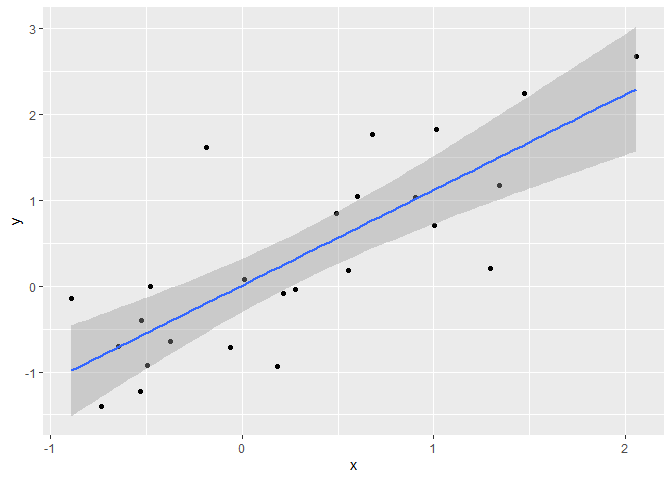
\includegraphics{561_Notes_files/figure-latex/Spurious Correlation-1.pdf}

\begin{Shaded}
\begin{Highlighting}[]
\CommentTok{# Distribution of all the correlations}
\NormalTok{res }\OperatorTok\StringTok{ }\KeywordTok{ggplot}\NormalTok{(}\KeywordTok{aes}\NormalTok{(}\DataTypeTok{x=}\NormalTok{r)) }\OperatorTok{+}\StringTok{ }\KeywordTok{geom_histogram}\NormalTok{(}\DataTypeTok{binwidth =} \FloatTok{0.1}\NormalTok{, }\DataTypeTok{color =} \StringTok{"black"}\NormalTok{)}
\end{Highlighting}
\end{Shaded}

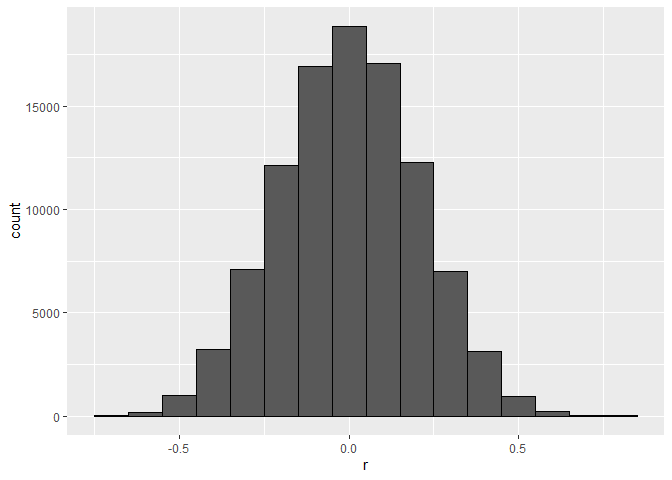
\includegraphics{561_Notes_files/figure-latex/Spurious Correlation-2.pdf}
\textgreater{} If we performed regression on the highly correlated group
and interpreted the p-value, we would incorrectly claim this was a
statistically significant relation. This particular form of data
dredging is referred to as p-hacking.

\hypertarget{outliers}{%
\paragraph{Outliers}\label{outliers}}

\begin{quote}
Suppose we take measurements from two independent outcomes, X and Y, and
we standardize the measurements. However, imagine we make a mistake and
forget to standardize entry 23. We can simulate such data using:
\end{quote}

\begin{Shaded}
\begin{Highlighting}[]
\KeywordTok{set.seed}\NormalTok{(}\DecValTok{1985}\NormalTok{)}
\NormalTok{x <-}\StringTok{ }\KeywordTok{rnorm}\NormalTok{(}\DecValTok{100}\NormalTok{,}\DecValTok{100}\NormalTok{,}\DecValTok{1}\NormalTok{)}
\NormalTok{y <-}\StringTok{ }\KeywordTok{rnorm}\NormalTok{(}\DecValTok{100}\NormalTok{,}\DecValTok{84}\NormalTok{,}\DecValTok{1}\NormalTok{)}
\NormalTok{x[}\OperatorTok{-}\DecValTok{23}\NormalTok{] <-}\StringTok{ }\KeywordTok{scale}\NormalTok{(x[}\OperatorTok{-}\DecValTok{23}\NormalTok{])}
\NormalTok{y[}\OperatorTok{-}\DecValTok{23}\NormalTok{] <-}\StringTok{ }\KeywordTok{scale}\NormalTok{(y[}\OperatorTok{-}\DecValTok{23}\NormalTok{])}

\KeywordTok{qplot}\NormalTok{(x, y)}
\end{Highlighting}
\end{Shaded}

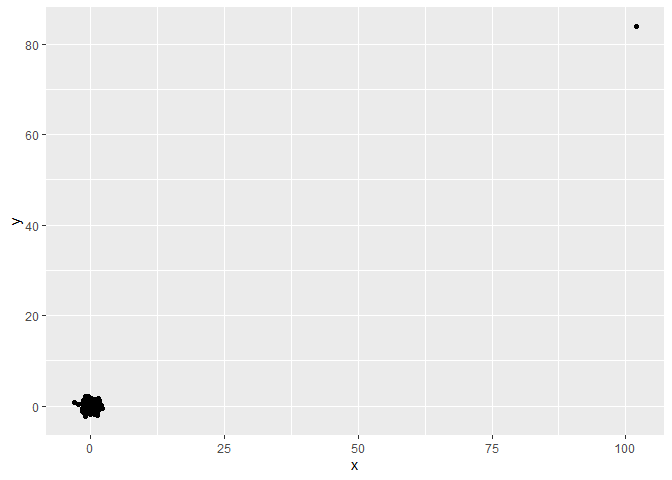
\includegraphics{561_Notes_files/figure-latex/Outliers-1.pdf}

\begin{Shaded}
\begin{Highlighting}[]
\KeywordTok{cor}\NormalTok{(x,y)}
\end{Highlighting}
\end{Shaded}

\begin{verbatim}
## [1] 0.9878382
\end{verbatim}

\begin{Shaded}
\begin{Highlighting}[]
\CommentTok{# But this is driven by the one outlier. If we remove this outlier, the correlation is greatly reduced to almost 0, which is what it should be:}

\KeywordTok{cor}\NormalTok{(x[}\OperatorTok{-}\DecValTok{23}\NormalTok{], y[}\OperatorTok{-}\DecValTok{23}\NormalTok{])}
\end{Highlighting}
\end{Shaded}

\begin{verbatim}
## [1] -0.04419032
\end{verbatim}

\begin{Shaded}
\begin{Highlighting}[]
\CommentTok{# an alternative to the sample correlation for estimating the population correlation that is robust to outliers. It is called Spearman correlation. The idea is simple: compute the correlation on the ranks of the values. Here is a plot of the ranks plotted against each other:}

\KeywordTok{qplot}\NormalTok{(}\KeywordTok{rank}\NormalTok{(x), }\KeywordTok{rank}\NormalTok{(y))}
\end{Highlighting}
\end{Shaded}

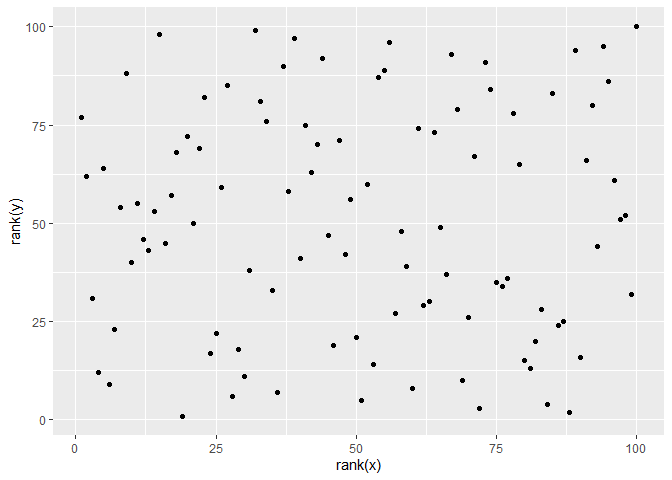
\includegraphics{561_Notes_files/figure-latex/Outliers-2.pdf}

\begin{Shaded}
\begin{Highlighting}[]
\CommentTok{# correlation}
\KeywordTok{cor}\NormalTok{(}\KeywordTok{rank}\NormalTok{(x), }\KeywordTok{rank}\NormalTok{(y))}
\end{Highlighting}
\end{Shaded}

\begin{verbatim}
## [1] 0.002508251
\end{verbatim}

\begin{Shaded}
\begin{Highlighting}[]
\KeywordTok{cor}\NormalTok{(x, y, }\DataTypeTok{method =} \StringTok{"spearman"}\NormalTok{)}
\end{Highlighting}
\end{Shaded}

\begin{verbatim}
## [1] 0.002508251
\end{verbatim}

\hypertarget{reversing-cause-and-effect}{%
\paragraph{Reversing cause and
effect}\label{reversing-cause-and-effect}}

\begin{itemize}
\tightlist
\item
  Another way association is confused with causation is when the cause
  and effect are reversed. An example of this is claiming that tutoring
  makes students perform worse because they test lower than peers that
  are not tutored. In this case, the tutoring is not causing the low
  test scores, but the other way around.
\item
  We can easily construct an example of cause and effect reversal using
  the father and son height data.
\end{itemize}

\begin{Shaded}
\begin{Highlighting}[]
\KeywordTok{library}\NormalTok{(HistData)}
\KeywordTok{data}\NormalTok{(}\StringTok{"GaltonFamilies"}\NormalTok{)}
\NormalTok{GaltonFamilies }\OperatorTok
\StringTok{  }\KeywordTok{filter}\NormalTok{(childNum }\OperatorTok{==}\StringTok{ }\DecValTok{1} \OperatorTok{&}\StringTok{ }\NormalTok{gender }\OperatorTok{==}\StringTok{ "male"}\NormalTok{) }\OperatorTok
\StringTok{  }\KeywordTok{select}\NormalTok{(father, childHeight) }\OperatorTok
\StringTok{  }\KeywordTok{rename}\NormalTok{(}\DataTypeTok{son =}\NormalTok{ childHeight) }\OperatorTok\StringTok{ }
\StringTok{  }\KeywordTok{do}\NormalTok{(}\KeywordTok{tidy}\NormalTok{(}\KeywordTok{lm}\NormalTok{(father }\OperatorTok{~}\StringTok{ }\NormalTok{son, }\DataTypeTok{data =}\NormalTok{ .)))}
\end{Highlighting}
\end{Shaded}

\begin{verbatim}
## # A tibble: 2 x 5
##   term        estimate std.error statistic  p.value
##   <chr>          <dbl>     <dbl>     <dbl>    <dbl>
## 1 (Intercept)   34.0      4.57        7.44 4.31e-12
## 2 son            0.499    0.0648      7.70 9.47e-13
\end{verbatim}

\begin{quote}
The model fits the data very well. If we look at the mathematical
formulation of the model above, it could easily be incorrectly
interpreted so as to suggest that the son being tall caused the father
to be tall. The model is technically correct. The estimates and p-values
were obtained correctly as well. What is wrong here is the
interpretation.
\end{quote}

\hypertarget{confounding}{%
\paragraph{Confounding}\label{confounding}}

\begin{itemize}
\tightlist
\item
  Confounders are perhaps the most common reason that leads to
  associations begin misinterpreted. If X and Y are correlated, we call
  Z a confounder if changes in Z causes changes in both X and Y.
\end{itemize}

\begin{quote}
Admission data from six U.C. Berkeley majors, from 1973, showed that
more men were being admitted than women: 44\% men were admitted compared
to 30\% women.
\end{quote}

\begin{Shaded}
\begin{Highlighting}[]
\KeywordTok{library}\NormalTok{(HistData)}
\KeywordTok{data}\NormalTok{(admissions)}
\NormalTok{admissions }\OperatorTok\StringTok{ }\KeywordTok{group_by}\NormalTok{(gender) }\OperatorTok\StringTok{ }
\StringTok{  }\KeywordTok{summarize}\NormalTok{(}\DataTypeTok{total_admitted =} \KeywordTok{round}\NormalTok{(}\KeywordTok{sum}\NormalTok{(admitted }\OperatorTok{/}\StringTok{ }\DecValTok{100} \OperatorTok{*}\StringTok{ }\NormalTok{applicants)), }
            \DataTypeTok{not_admitted =} \KeywordTok{sum}\NormalTok{(applicants) }\OperatorTok{-}\StringTok{ }\KeywordTok{sum}\NormalTok{(total_admitted)) }\OperatorTok
\StringTok{  }\KeywordTok{select}\NormalTok{(}\OperatorTok{-}\NormalTok{gender) }\OperatorTok\StringTok{ }
\StringTok{  }\KeywordTok{do}\NormalTok{(}\KeywordTok{tidy}\NormalTok{(}\KeywordTok{chisq.test}\NormalTok{(.))) }\OperatorTok\StringTok{ }\NormalTok{.}\OperatorTok{$}\NormalTok{p.value}
\end{Highlighting}
\end{Shaded}

But closer inspection shows a paradoxical result. Here are the percent
admissions by major:

\begin{Shaded}
\begin{Highlighting}[]
\NormalTok{admissions }\OperatorTok\StringTok{ }\KeywordTok{select}\NormalTok{(major, gender, admitted) }\OperatorTok
\StringTok{  }\KeywordTok{spread}\NormalTok{(gender, admitted) }\OperatorTok
\StringTok{  }\KeywordTok{mutate}\NormalTok{(}\DataTypeTok{women_minus_men =}\NormalTok{ women }\OperatorTok{-}\StringTok{ }\NormalTok{men)}
\end{Highlighting}
\end{Shaded}

\begin{quote}
The paradox is that analyzing the totals suggests a dependence between
admission and gender, but when the data is grouped by major, this
dependence seems to disappear. This actually can happen if an uncounted
confounder is driving most of the variability.
\end{quote}

\begin{quote}
Plot the total percent admitted to a major versus the percent of women
that made up the applicants:
\end{quote}

\begin{Shaded}
\begin{Highlighting}[]
\NormalTok{admissions }\OperatorTok\StringTok{ }
\StringTok{  }\KeywordTok{group_by}\NormalTok{(major) }\OperatorTok\StringTok{ }
\StringTok{  }\KeywordTok{summarize}\NormalTok{(}\DataTypeTok{major_selectivity =} \KeywordTok{sum}\NormalTok{(admitted }\OperatorTok{*}\StringTok{ }\NormalTok{applicants)}\OperatorTok{/}\KeywordTok{sum}\NormalTok{(applicants),}
            \DataTypeTok{percent_women_applicants =} \KeywordTok{sum}\NormalTok{(applicants }\OperatorTok{*}\StringTok{ }\NormalTok{(gender}\OperatorTok{==}\StringTok{"women"}\NormalTok{)) }\OperatorTok{/}
\StringTok{                                             }\KeywordTok{sum}\NormalTok{(applicants) }\OperatorTok{*}\StringTok{ }\DecValTok{100}\NormalTok{) }\OperatorTok
\StringTok{  }\KeywordTok{ggplot}\NormalTok{(}\KeywordTok{aes}\NormalTok{(major_selectivity, percent_women_applicants, }\DataTypeTok{label =}\NormalTok{ major)) }\OperatorTok{+}
\StringTok{  }\KeywordTok{geom_text}\NormalTok{()}
\end{Highlighting}
\end{Shaded}

\begin{itemize}
\tightlist
\item
  The plot suggests that women were much more likely to apply to the two
  ``hard'' majors. Gender and major's selectivity are confounded.
  \href{https://rafalab.github.io/dsbook/association-is-not-causation.html}{create
  a facet plot as shown in the book 19.4.2}
\item
  The majority of accepted men came from two majors: A and B. Few women
  applied to these majors.
\end{itemize}

\begin{quote}
Controlling the confounder
\end{quote}

\begin{Shaded}
\begin{Highlighting}[]
\NormalTok{admissions }\OperatorTok\StringTok{ }
\StringTok{  }\KeywordTok{ggplot}\NormalTok{(}\KeywordTok{aes}\NormalTok{(major, admitted, }\DataTypeTok{col =}\NormalTok{ gender, }\DataTypeTok{size =}\NormalTok{ applicants)) }\OperatorTok{+}
\StringTok{  }\KeywordTok{geom_point}\NormalTok{()}
\NormalTok{admissions }\OperatorTok\StringTok{  }\KeywordTok{group_by}\NormalTok{(gender) }\OperatorTok\StringTok{ }\KeywordTok{summarize}\NormalTok{(}\DataTypeTok{average =} \KeywordTok{mean}\NormalTok{(admitted))}
\end{Highlighting}
\end{Shaded}

If we average the difference by major, we find that the percent is
actually 3.5\% higher for women.

\begin{quote}
Confounding is addressed by adding the counfounding variable in the
model
\end{quote}

\hypertarget{example-of-confounding-simpsons-paradox}{%
\subparagraph{Example of Confounding Simpson's
Paradox}\label{example-of-confounding-simpsons-paradox}}

You can see that X and Y are negatively correlated. However, once we
stratify by Z (shown in different colors below) another pattern emerges:

\begin{figure}
\centering
\includegraphics{C:/MyDisk/MDS/simpsons_paradox.PNG}
\caption{simpsons\_paradox}
\end{figure}

\begin{quote}
It is really Z that is negatively correlated with X. If we stratify by
Z, the X and Y are actually positively correlated as seen in the plot
above.
\end{quote}

\begin{center}\rule{0.5\linewidth}{\linethickness}\end{center}

\begin{itemize}
\tightlist
\item
  \(R^2=\frac{ESS}{TSS}\) is always positive
\item
  \(R^2=1-\frac{RSS}{TSS}\) is not always positive, RSS can be larger
  the TSS when the model does not have intercept or not LS estimates
\item
  \((cor(y,\hat{y}))^2=R^2\), For a SLR model estimated by LS this is
  true, but it's \emph{not} true in general
\item
  Although the \(R^2\) compares the RSS of the \emph{full model} vs
  those of the \emph{null model}, it does not really tell us how good
  our model \emph{predicts}\\
\item
  The mean square error of prediction (PMSE) measures the distance
  between the predicted and the observed response

  \begin{itemize}
  \tightlist
  \item
    Can estimate both in-sample \& out-sample\\
  \item
    PMSE should be used to compare predicted with actual and not
    correlation as it can be confounded.\\
  \end{itemize}
\item
  Both the \(R^2\) and the \emph{F}-test are based on \emph{in-sample}
  predictions and does not give a measure of accuracy in new test
  samples
\end{itemize}

We compute Bootstrapping or Permutation to HT for the LS estimates: they
can be used if we believe the sample size is too small to trust
asymptotic results. These tests can be used for other estimators as
well.

\hypertarget{permutation-test-for-regression}{%
\paragraph{Permutation test for
regression}\label{permutation-test-for-regression}}

\begin{itemize}
\tightlist
\item
  We need to generate samples from the null hypothesis!!
  \(H_0: \beta_g=0\)
\item
  Steps:

  \begin{enumerate}
  \def\labelenumi{\arabic{enumi}.}
  \tightlist
  \item
    Shuffle the rows of \(X\) and combine them with the observed \(y\)
  \item
    Compute the estimate in the permuted sample
  \item
    Repeat 1-2 many times (\(B\))
  \item
    Compute the
    \(\text{p-value}=2 \times \frac{\#[\hat{\beta}^*> \hat{\beta}]}{B}\)
  \end{enumerate}
\end{itemize}

\hypertarget{bootstrapping-tests-for-regression}{%
\paragraph{Bootstrapping tests for
regression}\label{bootstrapping-tests-for-regression}}

\begin{itemize}
\tightlist
\item
  There are 2 types of resampling: (\(x\)-random) \& (\(x\)-fix). Only
  (\(x\)-random) is discussed\\
\item
  In classical tests the statistic is:
  \(T=\frac{\hat{\beta}-\beta_{H_0}}{\text{SE}[\hat{\beta}]}=\frac{\hat{\beta}-0}{\text{SE}[\hat{\beta}]}\)\\
\item
  The bootstrap statistic:
  \(T^*=\frac{\beta^*-\hat{\beta}}{\text{SE}[\beta^*]}\), get \(B\) of
  these!\\
\item
  pval: \(\frac{1+\#[|T^*| > |T|]}{B+1}\) to test \(H_0:\beta_1=0\) vs
  \(H_A: \beta_1 \neq 0\)\\
\item
  pval: \(\frac{1+\#[T^* > T]}{B+1}\) to test \(H_0:\beta_1=0\) vs
  \(H_A: \beta_1 > 0\)
\end{itemize}

\begin{Shaded}
\begin{Highlighting}[]
\CommentTok{# generate sample}
\NormalTok{n <-}\StringTok{ }\DecValTok{200} \CommentTok{# small n will result in skewed sampling distribution, high value will give more normal distribution (by CLT), but note that residuals are always non-normal, regardless of n}
\NormalTok{x <-}\StringTok{  }\KeywordTok{seq}\NormalTok{(}\DecValTok{1}\NormalTok{, n)}
\NormalTok{y <-}\StringTok{ }\NormalTok{x }\OperatorTok{+}\StringTok{ }\KeywordTok{rlnorm}\NormalTok{(n)}\OperatorTok{*}\NormalTok{x}
\NormalTok{df <-}\StringTok{ }\KeywordTok{tibble}\NormalTok{(}\DataTypeTok{x =}\NormalTok{ x, }\DataTypeTok{y =}\NormalTok{ y)}
\NormalTok{model <-}\StringTok{ }\KeywordTok{lm}\NormalTok{(y }\OperatorTok{~}\StringTok{ }\NormalTok{x, }\DataTypeTok{data =}\NormalTok{ df)}
\NormalTok{df <-}\StringTok{ }\NormalTok{df }\OperatorTok\StringTok{ }
\StringTok{  }\KeywordTok{mutate}\NormalTok{(}\DataTypeTok{resid =} \KeywordTok{predict}\NormalTok{(model) }\OperatorTok{-}\StringTok{ }\NormalTok{y)}
\CommentTok{# generate bootstrap sampling distribution for beta_1}
\NormalTok{N <-}\StringTok{ }\DecValTok{1000}
\NormalTok{boot_fits <-}\StringTok{ }\NormalTok{df }\OperatorTok\StringTok{ }
\StringTok{    }\NormalTok{rsample}\OperatorTok{::}\KeywordTok{bootstraps}\NormalTok{(}\DataTypeTok{times =}\NormalTok{ N) }\OperatorTok\StringTok{ }
\StringTok{    }\KeywordTok{mutate}\NormalTok{(}
        \DataTypeTok{lm   =} \KeywordTok{map}\NormalTok{(splits, }\OperatorTok{~}\StringTok{ }\KeywordTok{lm}\NormalTok{(y }\OperatorTok{~}\StringTok{ }\NormalTok{x, }\DataTypeTok{data =} \KeywordTok{analysis}\NormalTok{(.x))),}
        \DataTypeTok{tidy =} \KeywordTok{map}\NormalTok{(lm, broom}\OperatorTok{::}\NormalTok{tidy) }
\NormalTok{    ) }\OperatorTok\StringTok{ }
\StringTok{    }\KeywordTok{select}\NormalTok{(}\OperatorTok{-}\NormalTok{splits, }\OperatorTok{-}\NormalTok{lm) }\OperatorTok\StringTok{ }
\StringTok{    }\KeywordTok{unnest}\NormalTok{(tidy) }\OperatorTok\StringTok{ }
\StringTok{    }\KeywordTok{filter}\NormalTok{(term }\OperatorTok{==}\StringTok{ "x"}\NormalTok{) }\OperatorTok\StringTok{ }
\StringTok{    }\KeywordTok{select}\NormalTok{(}\OperatorTok{-}\NormalTok{term)}

\CommentTok{# plot bootstrap sampling distribution for beta_1}
\KeywordTok{ggplot}\NormalTok{(boot_fits, }\KeywordTok{aes}\NormalTok{(estimate)) }\OperatorTok{+}
\StringTok{    }\KeywordTok{geom_histogram}\NormalTok{(}\DataTypeTok{bins =} \DecValTok{30}\NormalTok{, }\DataTypeTok{color=}\StringTok{"black"}\NormalTok{, }\DataTypeTok{fill=}\StringTok{"white"}\NormalTok{) }\OperatorTok{+}
\StringTok{  }\KeywordTok{ggtitle}\NormalTok{(}\StringTok{'Bootstrap sampling distribution'}\NormalTok{) }\OperatorTok{+}
\StringTok{  }\KeywordTok{labs}\NormalTok{(}\DataTypeTok{x =} \KeywordTok{expression}\NormalTok{(Estimate}\OperatorTok{~}\NormalTok{of}\OperatorTok{~}\NormalTok{beta[}\DecValTok{1}\NormalTok{])) }
\end{Highlighting}
\end{Shaded}

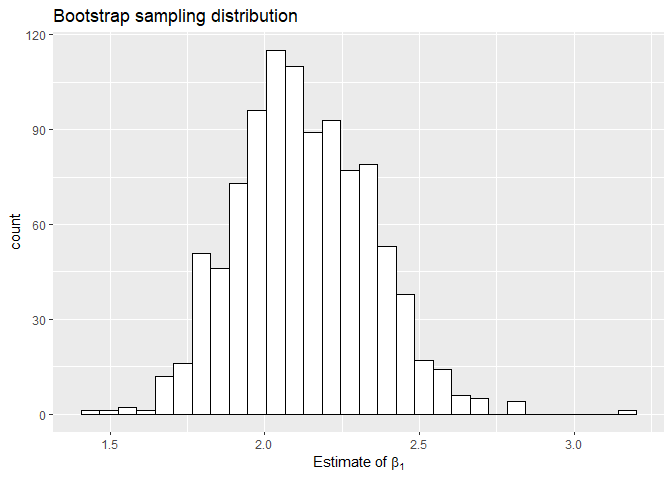
\includegraphics{561_Notes_files/figure-latex/models-1.pdf}

\begin{Shaded}
\begin{Highlighting}[]
\NormalTok{b_obs <-}\StringTok{ }\KeywordTok{tidy}\NormalTok{(model)  }\OperatorTok\StringTok{ }\KeywordTok{filter}\NormalTok{(term }\OperatorTok{==}\StringTok{ "x"}\NormalTok{) }\OperatorTok\StringTok{ }\KeywordTok{select}\NormalTok{(estimate, statistic,p.value) }

\NormalTok{t_star <-}\StringTok{ }\KeywordTok{data.frame}\NormalTok{(}\DataTypeTok{t_star=}\NormalTok{(boot_fits}\OperatorTok{$}\NormalTok{estimate }\OperatorTok{-}\StringTok{ }\NormalTok{b_obs}\OperatorTok{$}\NormalTok{estimate)}\OperatorTok{/}\NormalTok{boot_fits}\OperatorTok{$}\NormalTok{std.error)}

\CommentTok{#pval using t-distribution}
\NormalTok{pval_t<-b_obs}\OperatorTok{$}\NormalTok{p.value}
\KeywordTok{print}\NormalTok{(}\KeywordTok{paste}\NormalTok{(}\StringTok{"pval using t-distribution"}\NormalTok{, pval_t))}
\end{Highlighting}
\end{Shaded}

\begin{verbatim}
## [1] "pval using t-distribution 1.94285241567769e-21"
\end{verbatim}

\begin{Shaded}
\begin{Highlighting}[]
\CommentTok{#pval using bootstrapping and pivot method}
\NormalTok{pval_boot <-}\StringTok{ }\NormalTok{(}\DecValTok{1}\OperatorTok{+}\KeywordTok{sum}\NormalTok{(}\KeywordTok{abs}\NormalTok{(t_star) }\OperatorTok{>}\StringTok{ }\KeywordTok{abs}\NormalTok{(b_obs}\OperatorTok{$}\NormalTok{statistic)))}\OperatorTok{/}\NormalTok{(N}\OperatorTok{+}\DecValTok{1}\NormalTok{)}
\KeywordTok{print}\NormalTok{(}\KeywordTok{paste}\NormalTok{(}\StringTok{"pval using bootstrapping and pivot method"}\NormalTok{, pval_boot))}
\end{Highlighting}
\end{Shaded}

\begin{verbatim}
## [1] "pval using bootstrapping and pivot method 0.000999000999000999"
\end{verbatim}

\begin{center}\rule{0.5\linewidth}{\linethickness}\end{center}

\begin{itemize}
\tightlist
\item
  The conditional expectation is the best predictor of 𝑌 given a vector
  of variables 𝑋
\item
  A LM can be used as a predictor but it may not be the best
\item
  If the data is jointly normal, the best predictor is linear!!
\item
  The least squares regression is the best among other linear predictors
\end{itemize}

\begin{center}\rule{0.5\linewidth}{\linethickness}\end{center}

\begin{itemize}
\tightlist
\item
  Let's only assume that the errors are \(iid\) (independent and
  identically distributed) and independent of \(X_j\)

  \begin{itemize}
  \tightlist
  \item
    with \(E[\varepsilon_i]=0\) and \(Var(\varepsilon_i)=\sigma\)\\
  \end{itemize}
\item
  Note that this assumption implies that
  \(E[Y|\mathbf{X}]=\beta_0 + \beta_1 X_{i1} + \ldots + \beta_p X_{ip}\)

  \begin{itemize}
  \tightlist
  \item
    this is just an assumption!! it's true under normality but we are
    not assuming that (yet)\\
  \end{itemize}
\item
  Note that we are \textbf{\emph{not assuming}} that
  \(\varepsilon_i \sim \mathcal{N}(0,\sigma)\)
\end{itemize}

\hypertarget{ls-estimator}{%
\subsubsection{LS estimator}\label{ls-estimator}}

\begin{itemize}
\tightlist
\item
  Find \(\beta_0, \beta_1, \ldots, \beta_p\) that minimizes the sum of
  squared errors:
  \(\sum_i^n(Y_i - \beta_0 - \beta_1 X_{i1} - \ldots - \beta_p X_{ip})^2\)\\
\item
  The minimizer is the LS estimator :
  \(\hat{\beta}_0, \hat{\beta}_1, \ldots, \hat{\beta}_p\)
\end{itemize}

\hypertarget{properties-of-the-ls-estimator}{%
\paragraph{Properties of the LS
estimator:}\label{properties-of-the-ls-estimator}}

\begin{itemize}
\tightlist
\item
  Unbiased estimator meaning,
  \(E[\hat{\mathbf{\beta}}]=\mathbf{\beta}\)\\
\item
  Best (lowest variance) Linear Unbiased Estimator
\item
  \(Var(\hat{\mathbf{\beta}})=\sigma^2(\mathbf{X}^T\mathbf{X})^{-1}, \; \hat{\sigma}=\sqrt{\frac{\sum_{i=1}^n\hat{e}_i^2}{n-p-1}}\)
  (\(p\) slopes + 1 intercept)

  \begin{itemize}
  \tightlist
  \item
    \texttt{sig\_hat\ \textless{}-\ augment(lm\_s,\ dat\_s)\ \ \%\textgreater{}\%\ select(.resid)\ \ \%\textgreater{}\%\ summarize(sig\_hat=\ sqrt(sum(.resid\^{}2)/(length(.resid)-2)))}
  \end{itemize}
\item
  This is the estimate given by \texttt{lm}!!
\item
  The mean squared error for the estimator, not the prediction:

  \begin{itemize}
  \tightlist
  \item
    \(\text{MSE}(\hat{\beta})=E[(\hat{\beta}-\beta)^2]= Var(\hat{\beta})+\text{Bias}(\hat{\beta})^2= Var(\hat{\beta})+(E(\hat{\beta})-\beta)^2\)
  \end{itemize}
\end{itemize}

\hypertarget{matrix-notation-of-the-lienar-model}{%
\paragraph{Matrix Notation of the lienar
model:}\label{matrix-notation-of-the-lienar-model}}

\hypertarget{we-want-to-minimize-squared-error}{%
\paragraph{We want to minimize squared
error:}\label{we-want-to-minimize-squared-error}}

\begin{itemize}
\tightlist
\item
  \(S(\beta_0,\beta_1,\beta_2)=\mathbf{\varepsilon}^T\mathbf{\varepsilon}=(\mathbf{Y}- \mathbf{X} \mathbf{\beta})^T (\mathbf{Y} - \mathbf{X} \mathbf{\beta})\)\\
\item
  \(\frac{\partial{S}}{\partial{\mathbf{\beta}}}=\mathbf{0}= -2\mathbf{X}^T(\mathbf{Y}-\mathbf{X}\mathbf{\beta}) \iff \mathbf{X}^T\mathbf{X}\hat{\mathbf{\beta}}=\mathbf{X}^T\mathbf{Y}\)\\
\item
  \(\hat{\mathbf{\beta}}=(\mathbf{X}^T\mathbf{X})^{-1}\mathbf{X}^T\mathbf{Y}\)\\
\item
  Note that I \emph{never} assume a distribution for \(\varepsilon\).
  the errors does not have to be Normal!!
\item
  Given \(\mathbf{X}\), \(\hat{\mathbf{\beta}}\) is a linear function of
  \(\mathbf{Y}\), and \(\mathbf{Y}\) has the same distribution as
  \(\varepsilon_i\)
\item
  If
  \(\varepsilon_i \sim \mathcal{N}(0,\sigma^2) \implies \hat{\mathbf{\beta}}\)
  is also Normal!! and we can construct an exact tests for the model
  coefficients
\item
  \(\hat{\beta}_1 \sim \mathcal{N}\left(\beta_1,\frac{\sigma^2}{(n-1)s_x^2}\right) \implies \quad z=\frac{\hat{\beta}_1-\beta_1}{SE(\hat{\beta}_1)}=\frac{\hat{\beta}_1-\beta_1}{\frac{\sigma}{\sqrt{(n-p-1)s^2_x}}} \sim \mathcal{N}(0,1)\)
\item
  Since \(\sigma\) is usually \emph{unknown}:
  \(t=\frac{\hat{\beta}_1-\beta_1}{SE(\hat{\beta}_1)}=\frac{\hat{\beta}_1-\beta_1}{\frac{\hat{\sigma}}{\sqrt{(n-1)s^2_x}}} \sim \mathcal{t}_{n-p-1}\)
\end{itemize}

\hypertarget{what-if-varepsilon_i-are-not-normal}{%
\paragraph{\texorpdfstring{What if \(\varepsilon_i\) are
\textbf{\emph{not}}
Normal??}{What if \textbackslash{}varepsilon\_i are not Normal??}}\label{what-if-varepsilon_i-are-not-normal}}

\begin{itemize}
\tightlist
\item
  According to Central Limit Theorem, It can be proved that under
  certain conditions, the \emph{asymptotic} sampling distribution of the
  LS estimators is \emph{normal}, even when the errors are not!!.
  However, this result requires a large sample size (and ``large''
  depends on characteristics of the sample).\\
\item
  \texttt{lm} uses this result and constructs a \emph{t}-statistic under
  the null hypothesis \(H_0: \beta_j=0\) with
  \(t=\frac{\hat{\beta}_j-0}{SE(\hat{\beta}_j)}\sim \mathcal{t}_{n-p-1}\)
\end{itemize}

\hypertarget{confidence-intervals-for-prediction-cip}{%
\paragraph{Confidence Intervals for Prediction
(CIP)}\label{confidence-intervals-for-prediction-cip}}

\begin{itemize}
\tightlist
\item
  Example: ``Are you predicting the average value of a house with the
  given dimensions?''
\item
  The fitted value, \(\hat{Y}\) (random variable) predicts the true
  value of conditional expectation of Y given X\\
\item
  There is only 1 sources of variation for this prediction: the
  uncertainty of the estimated coefficients\\
\item
  \(\hat{Y}(x^*) \pm t_{n-2,0.975} \times SE_{\hat{\mu}_{Y|x^*}}; \; SE_{\hat{\mu}_{Y|x^*}}=\hat{\sigma} \sqrt{\frac{1}{n}+\frac{(x^*-\bar{x})^2}{(n-1)s_x^2}}\)
\item
  The \emph{t}-distribution here is derived from the conditional
  distribution of \(\varepsilon\) given \(\mathbf{X}\). Thus, there is
  no CLT that we can rely on!! This result is assuming normality of the
  error terms!!
\end{itemize}

\hypertarget{prediction-intervals-pi}{%
\paragraph{Prediction Intervals (PI)}\label{prediction-intervals-pi}}

\begin{itemize}
\tightlist
\item
  Example: ``Are you predicting the value of this given house that has
  these dimensions?''
\item
  The fitted value, \(\hat{Y}\) predicts the \emph{actual black
  point}.\\
\item
  There are 2 sources of variation: the uncertainty of the estimated
  coefficients \emph{and} that of the error that generates the data.\\
\item
  PI are wider than CI for prediction.\\
\item
  \(\hat{Y}(x^*) \pm t_{n-2,0.975} \times SE(\hat{Y}(x^*))\);
  \(SE(\hat{Y}(x^*))=\hat{\sigma} \sqrt{1+\frac{1}{n}+\frac{(x^*-\bar{x})^2}{(n-1)s_x^2}}\)
\end{itemize}

\hypertarget{mulitcollinearity}{%
\paragraph{Mulitcollinearity}\label{mulitcollinearity}}

\begin{itemize}
\tightlist
\item
  The least squares estimates satisfy:
  \(\mathbf{X}^T\mathbf{X}\hat{\mathbf{\beta}}=\mathbf{X}^T\mathbf{Y}\).
  If \(\mathbf{X}^T\mathbf{X}\) is non-singular (analogous to
  \(\neq 0\)), then
  \(\hat{\mathbf{\beta}}=(\mathbf{X}^T\mathbf{X})^{-1}\mathbf{X}^T\mathbf{Y}\)\\
\item
  However, \(\mathbf{X}^T\mathbf{X}\) becomes nearly singular or
  singular when explanatory variables are collinear or multicollinear,
  aka \emph{multicollinearity problem}.

  \begin{itemize}
  \tightlist
  \item
    the solution \((\mathbf{X}^T\mathbf{X})^{-1}\mathbf{X}^T\mathbf{Y}\)
    becomes very unstable!! (e.g., values and sign of some coefficients
    change as variables are added)\\
  \item
    \(Var(\hat{\mathbf{\beta}})=\sigma^2(\mathbf{X}^T\mathbf{X})^{-1}\)
    so the SEs of \(\hat{\mathbf{\beta}}\) can be large under
    multicollinearity\\
  \end{itemize}
\item
  Measured through the variance inflation factors (VIF):
  \(\text{VIF}_j=\frac{1}{1-R^2_{X_j,\boldsymbol{X}_{-j}}}, \; j=(1,\ldots,p)\)
  and \(R^2_{X_j,\boldsymbol{X}_{-j}}\) measures how much of the
  observed variation of \(X_j\) can be explained by other variables
\end{itemize}


\end{document}
